\label{sec:SRpart1}

\section{Sparse regularization}

\subsection{Denoising} Surfaces obtained through a scanning process or other reconstruction algorithm are inevitably noisy, even when using high-fidelity scanners, so mesh denoising is an important tool in geometry processing to remove the noise from the input data. A wide variety of denoising algorithms have already been proposed that mainly can be divided into two approaches: prescribed differential information based and extending the bilateral filter from 2D signal processing to arbitrary 3D meshes. But it is inherently challenging as it can be difficult to distinguish features from noise.

\paragraph{(1)} In image processing, \cite{xu2011image} aiming to smooth images provides an algorithm for directly optimizing the $L_0$ norm to create piecewise constant images. Let $c$ be a vector of pixel colors and $\triangledown c$ be a vector of gradients of these colors. The authors get the smoothed image by minimizing $|c-c^{*}|^2+|\triangledown c|_0$ where $|\triangledown c|_0$ is the $L_0$ norm of $\triangledown c$ and $c^{*}$ represents the original image colors to provide a data fidelity term.

A natural extension to triangulated meshes is to design a discrete differential operator to replace $\triangledown c$ that is zero when the surface is flat for arbitrary triangulations irrespective of the rotation or translation of the surface. 
This constraint implies that some form of second order information rather than the first order in formation provided by $\triangledown c$ is needed, e.g.,  the discrete Laplacian operator\cite{pinkall1993computing} which is computed as a weighted combination of a vertex and its one-ring where the weights are given by cotangents of angles of the triangles.
However,\parpic[r]{\label{fig:failureLaplaciandenoise}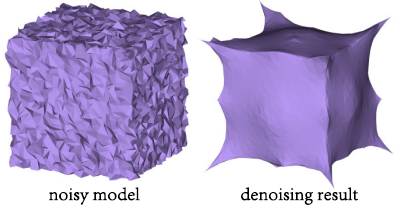
\includegraphics[width=0.6\linewidth]{images/denoise12}}the vertex-based Laplacian only constrains the mean curvature vector as opposed to a metric that directly measures sharpness per edge, then the optimization fails to reproduce sharp features and shrinks the surface away from the features shown as right.

\parpic[r]{\label{fig:edgeoperator}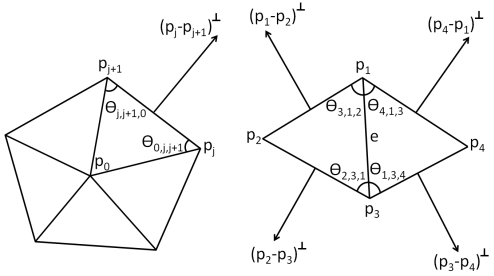
\includegraphics[width=0.6\linewidth]{images/denoise11}}
\cite{he2013mesh} generalizes the construction of the vertex-based cotan operator to an operator that acts directly on an edge

\small{
\begin{equation}
 \label{eq:edgecotanoperator}
 D(e) := {\left[ \begin{array}{c}
 \frac{\vartriangle_{1,2,3}((p_4-p_3)\cdot(p_3-p_1))}{\vartriangle_{1,3,4}((p_1-p_3)\cdot(p_3-p_2))} \\
 \frac{\vartriangle_{1,3,4}}{\vartriangle_{1,2,3}+\vartriangle_{1,3,4}} \\
 \frac{\vartriangle_{1,2,3}((p_3-p_1)\cdot(p_1-p_4))}{\vartriangle_{1,3,4}((p_2-p_1)\cdot(p_1-p_3))} \\
 \frac{\vartriangle_{1,2,3}}{\vartriangle_{1,2,3}+\vartriangle_{1,3,4}}
 \end{array}
 \right]}^{T}
 \left[ \begin{array}{c}
 p_1 \\ p_2 \\ p_3 \\ p_4
 \end{array}
 \right]
\end{equation}
}

Then the extended optimization problem is to make the edge operator sparse formulated as following

\small{
\begin{equation}
 \label{eq:edgecotanoperator}
 \min_{p,\delta}|p-p^{*}|^2+\alpha|R(p)|^2+\beta|D(p)-\delta|^2+\lambda|\delta|_0
\end{equation}
}
\\
where $p$ are the vertices of the shape, $p^{*}$ are their initial positions, $D(p)$ is a vector where the $i^{th}$ entry corresponds to the area-based edge operator applied to the $i^{th}$ edge, and $R(p)$ is a regularization term. Figure...gives one denoised result while preserving sharp features.

\begin{figure}[ht]
  \centering
  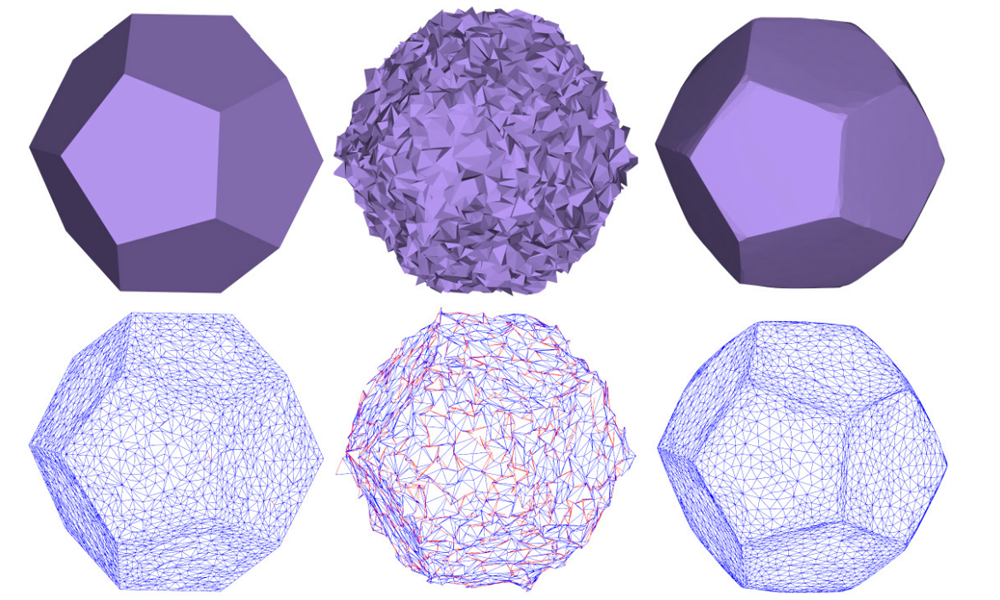
\includegraphics[width=2.5in]{images/denoise1}
  \caption{Sparse regularization: mesh denoising\cite{he2013mesh}. Left: initial surface. Center: surface corrupted by Gaussian noise in random directions with standard deviation $\sigma=0.4l_{e}$($l_{e}$ is the mean edge length). Right: denoising result. The wireframe shows folded triangles as red edges.}
\end{figure}

\begin{figure*}[ht]
  \centering
  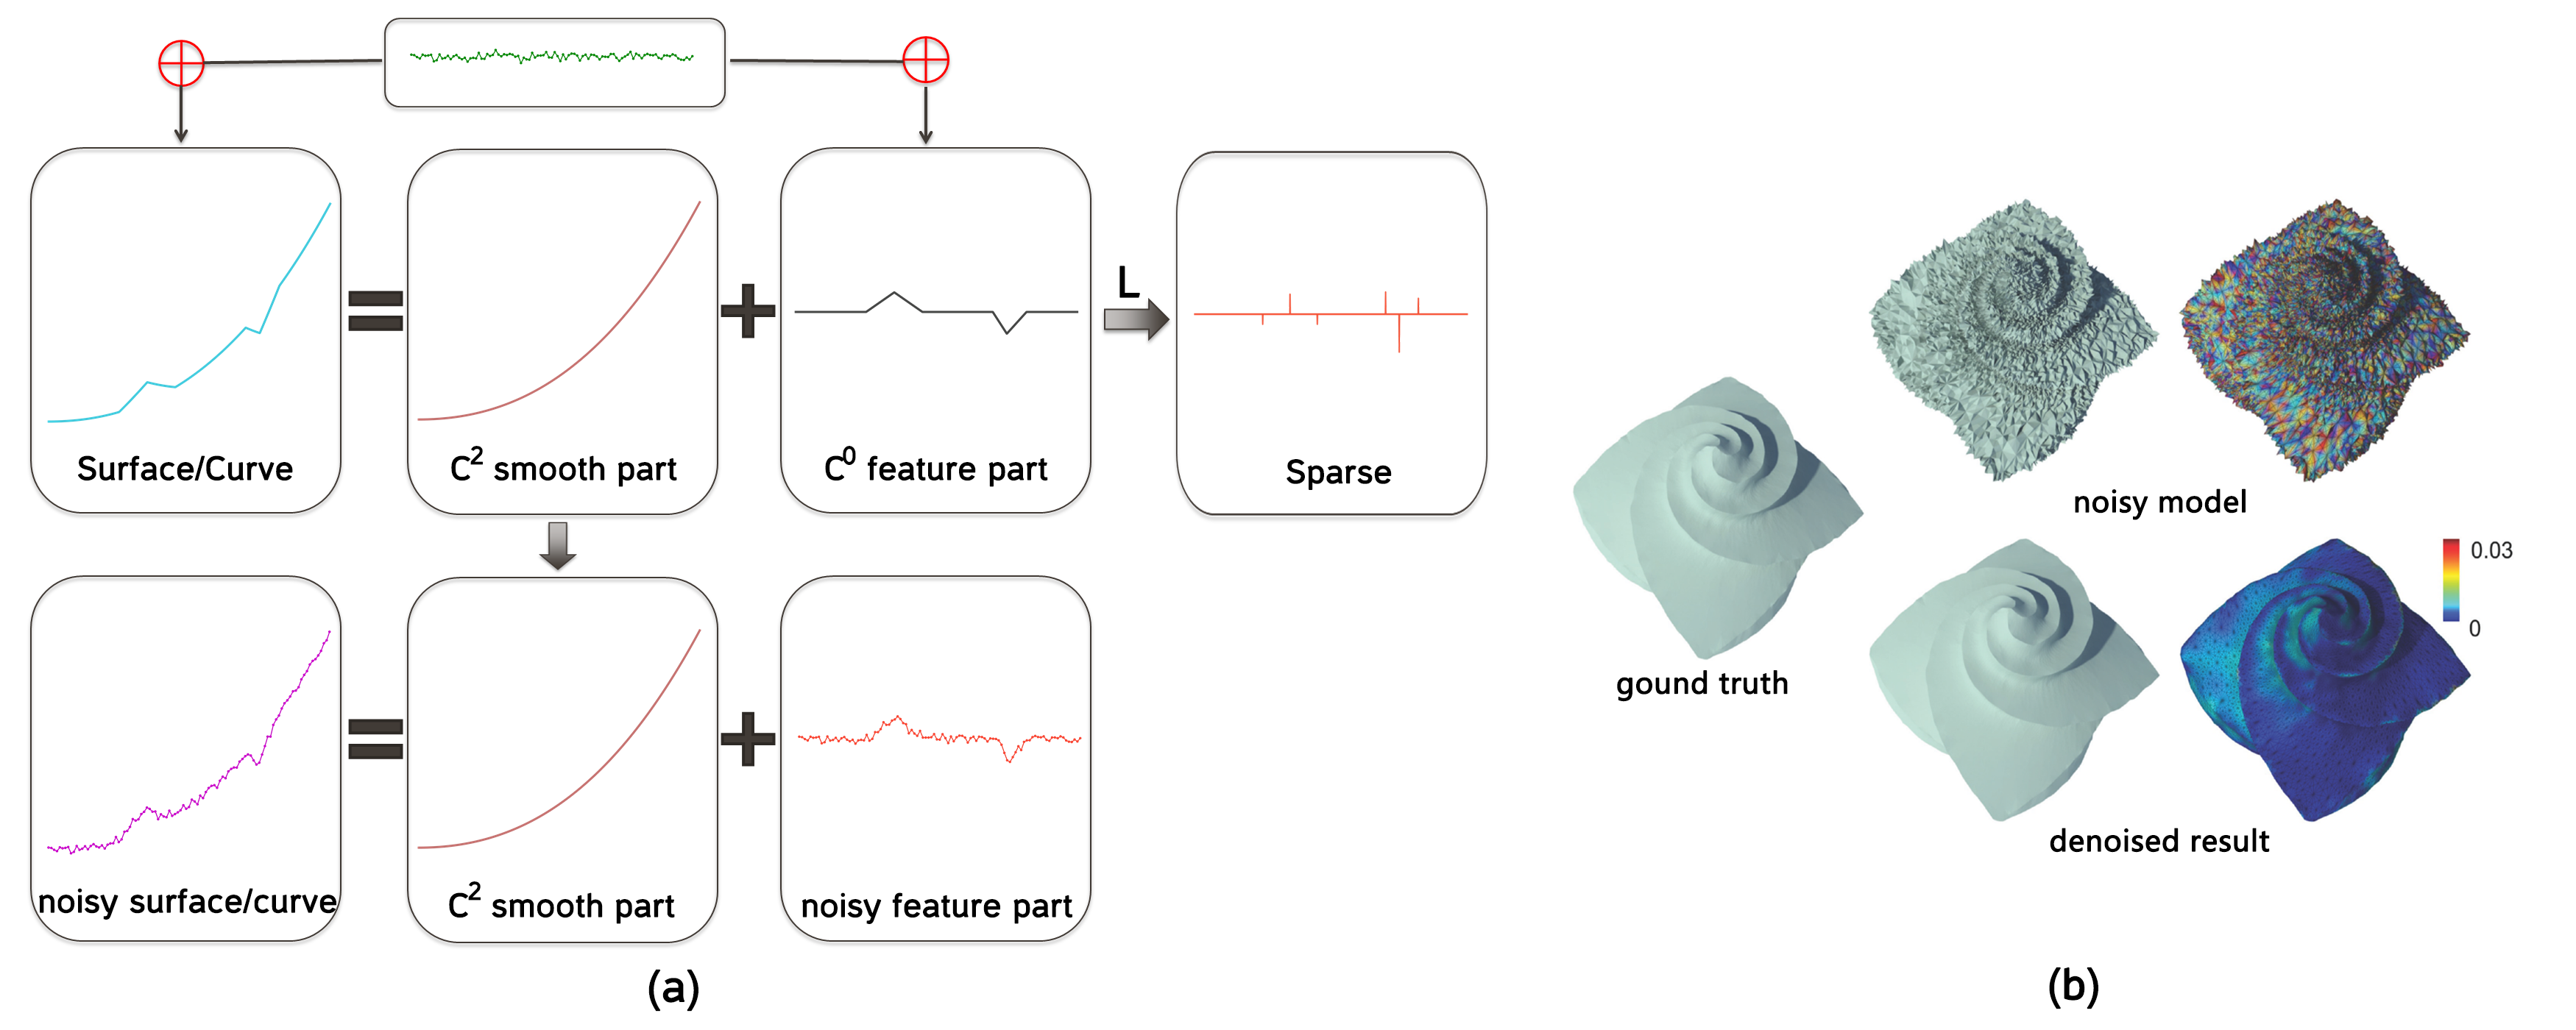
\includegraphics[width=5in]{images/denoise2_1}
  \caption{Sparse regularization: mesh denoising\cite{wang2014decoupling}. (a) is the two-dimensional illustration for their key observation. (b) is a denoising example.}
\end{figure*}

\paragraph{(2)}
Like most previous methods, how to tune the parameters shown in () has not theoretical guarantee and the computation of differential properties for detecting noise from feature is unreliable and unstable.

To address these problems, \cite{wang2014decoupling} presents a two phase approach for decoupling features and noise on discrete surfaces to.
Figure..(a) gives a two-dimensional curve as illustrations of their key observation: any surface is piecewise $C^2$, that is, a surface consists of two parts: $C^2$ smooth part and $C^0$ feature part which can be transformed into a sparse signal by applying the Laplacian operator as mentioned above().
So the denoising problem is divided into two phase: smooth part(base mesh) estimation and recovering features from the corrupted feature part.

They firstly generate a base mesh by denoising the input data using a global Laplacian regularization smoothing optimization in which the smoothness parameter is automatically chosen by adopting the generalized cross-validation scheme,
then decouple the features $x$ and noises simultaneously from the noisy feature part $y$ via the $\ell_1$ analysis compressed sensing optimization

\small{
\begin{equation}
 \label{eq:edgecotanoperator}
 \min_{x}\|Lx\|_1~~ s.t. ~ \|y-x\|_2 \le \epsilon
\end{equation}
}

Finally combining the resulted feature part and the previous obtained base mesh will reduce the final result. It is the first time noise and features are analyzed and separated in such an elegant manner with guarantees by statistical theory which is exciting and sightworthy in the smoothing optimization which is out of our scope. %But it works under some assumptions: independent and identically distributed(i.i.d.) noise and correct %connectivity information. 